\documentclass[times, 11pt]{article}
\usepackage[utf8]{inputenc}

\usepackage{graphicx}
\usepackage{amsmath, amsfonts, amssymb, mathrsfs, rotating, setspace,natbib}
\usepackage[left=1in,top=1in,right=1in,bottom=1in]{geometry}
%\renewcommand{\baselinestretch}{1.0}

\def \v{\mbox{Var}}
\def \E{\mathbb{E}}
\def \c{\mbox{Cov}}

\usepackage[usenames]{color}
\usepackage[colorlinks=true]{hyperref}
\hypersetup{linkcolor=blue,citecolor=blue,filecolor=black,urlcolor=blue} 

%% Please use the following statements for 
%% managing the text and math fonts for your papers:
\usepackage{times}
\usepackage{amsmath, amssymb, amsthm, mathrsfs}
\usepackage{rotating}

%\usepackage{graphicx}
%\usepackage[cmbold]{mathtime}

\usepackage{natbib}
\linespread{1.5}
%% user defined macros

\def \v{\mbox{Var}}
\def \E{\mathbb{E}}
\def \c{\mbox{Cov}}


\newcommand{\bmX}{\mbox{\boldmath $X$}}
%\newcommand{\hatb0}{\mbox{$\widehat{\beta}_0$}}
\newcommand{\bmY}{\mbox{\boldmath $Y$}}
\newcommand{\bmy}{\mbox{\boldmath $y$}}
\newcommand{\bmZ}{\mbox{\boldmath $Z$}}
\newcommand{\bmz}{\mbox{\boldmath $z$}}
\newcommand{\bmx}{\mbox{\boldmath $x$}}
\newcommand{\bmQ}{\mbox{\boldmath $Q$}}
\newcommand{\bmU}{\mbox{\boldmath $U$}}
\newcommand{\bmu}{\mbox{\boldmath $u$}}
\newcommand{\bmV}{\mbox{\boldmath $V$}}
\newcommand{\bmI}{\mbox{\boldmath $I$}}
\newcommand{\bmW}{\mbox{\boldmath $W$}}
\newcommand{\bmD}{\mbox{\boldmath $D$}}
\newcommand{\bms}{\mbox{\boldmath $s$}}
\newcommand{\bma}{\mbox{\boldmath $a$}}
\newcommand{\bmb}{\mbox{\boldmath $b$}}
\newcommand{\bmq}{\mbox{\boldmath $q$}}
\newcommand{\bmf}{\mbox{\boldmath $f$}}
\newcommand{\bmA}{\mbox{\boldmath $A$}}
%\newcommand{\bmepsilon}{\mbox{\boldmath $\epsilon$}}
\newcommand{\Prob}{\mbox{Pr}}
\newcommand{\bmone}{\mbox{\bf 1}}
\newcommand{\bmzero}{\mbox{\bf 0}}
\newcommand{\bmbeta}{\mbox{\boldmath $\beta$}}
\newcommand{\bmdelta}{\mbox{\boldmath $\delta$}}
\newcommand{\bmtheta}{\mbox{\boldmath $\theta$}}
\newcommand{\bmpsi}{\mbox{\boldmath $\psi$}}
\newcommand{\bmphi}{\mbox{\boldmath $\phi$}}
\newcommand{\bmnu}{\mbox{\boldmath $\nu$}}
\newcommand{\bmgamma}{\mbox{\boldmath $\gamma$}}
\newcommand{\bmmu}{\mbox{\boldmath $\mu$}}
\newcommand{\bmepsilon}{\mbox{\boldmath $\epsilon$}}
\newcommand{\bmSigma}{\mbox{\boldmath $\Sigma$}}

%\newtheorem{proposition}[theorem]{Proposition}
\begin{document}
\author{Erin E. Gabriel, Michael C. Sachs and Peter B. Gilbert}
\title{Comparing and Combining Biomarkers as Principle Surrogates for Time-to-Event Clinical Endpoints: Supplementary Materials}
\maketitle



\section{Web Appendix A}

\subsection{Non-random Group of Subjects with Candidate Surrogate Measurements}
To account for the possible biased sampling of $S_{j}(1)$, when case-cohort or two-phase sampling is used in the treatment arm to obtain $S_j(1)$ measurements, one can use inverse sampling probability weights in both the fitting of the location-scale model and the fitting of the imputed likelihood. Those with the candidate PS measured have their likelihood contribution unweighted, and each imputed likelihood contribution is weighted by the inverse probability of measurement for the $s_{1,j,k}$(s) giving rise to that imputation. Thus, the estimated likelihood contribution for subjects missing $S_{j}(1)$ is an inverse probability weighted average of their imputed likelihood contributions. When estimating the proposed summary statistics, an unbiased sample, as we have in our simulations and motivating example, allows for empirical estimation of integrals with respect to $F_{S_1(1), \ldots, S_J(1)}(s_{1,1}, \dots, s_{1,J})$. If the group of subjects with the candidate surrogates measured is not a random sample from the treatment arm, but the sample of subjects having W measured is we suggest Monte Carlo estimation of the integrals by sampling from the weighted location-scale estimated $d\hat{F}_{S_{1}(1),\ldots,S_{J}(1)|W}(s_{1,1},\ldots,s_{1,J}|W)$ across the observed levels of W. 


\subsection{Derivation of formula for $TPF(t|c)$}
\begin{eqnarray*}
TPF(t|c)&=&P[D(t)=1,\mathrm{I}_{\{\Delta(t|s_{1,1}, \dots, s_{1,J})>c\}}] \over P\{D(t)=1\}\\
&=&E[\{D(t)=1\}\mathrm{I}_{\{\Delta(t|s_{1,1}, \dots, s_{1,J})>c\}}] \over E\{D(t)=1\}\\
&=&{E[E\{D(t)=1|S_{1}(1)=s_{1,1}, \ldots, S_{j}(1)=s_{1,j}\}\mathrm{I}_{\{\Delta(t|s_{1,1}, \dots, s_{1,J})>c\}}] \over E[E\{D(t)=1|S_{1}(1)=s_{1,1}, \ldots, S_{j}(1)=s_{1,j}\}]}\\
&=&{E[\Delta(t|s_{1,1}, \dots, s_{1,J})\}\mathrm{I}_{\{\Delta(t|s_{1,1}, \dots, s_{1,J})>c\}}] \over E\{\Delta(t|s_{1,1}, \dots, s_{1,J})\}}.
\end{eqnarray*}
This deviation follows the time-independent derivation from \citet{Huang12b}.

\subsection{Violations of A6}
\begin{eqnarray*}
P(\Delta(t|s_{1,1}, \dots, s_{1,J})>c|D(t)=1)\frac{P(D(t)=1)}{P(D(t)=1)+P(D(t)=-1)}\\
-P(\Delta(t|s_{1,1}, \dots, s_{1,J})>c|D(t)=-1)\frac{P(D(t)=-1)}{P(D(t)=1)+P(D(t)=-1)}.
\end{eqnarray*}
When there are obvious violations of A6, this is clearly not a good approximation of what we hope to estimate in the non-monotone setting, the true positive fraction for benefit, as defined in \citet{Huang12b}, $TPF^{b}(t|c)=P(\Delta(t|s_{1,1}, \dots, s_{1,J})>c|D(t)=1)$. Thus, under clear violation of A6, the $TPF(t|c)$ estimate should not be calculated. Under minor potential undetectable violations of A6, $P(D(t)=-1)$ will be small and the estimator of $TPF(t|c)$ will be a reasonable approximation. For the slightly more complicated case of $FPF(t|c)$, the decomposition of the derivation under violation of A6 is given by:
\begin{eqnarray*}
&&P(\Delta(t|s_{1,1}, \dots, s_{1,J})>c|D(t)<1)\frac{P(D(t)<1)}{P(D(t)=-1)+P(D(t)<1)}\\
&-&P(\Delta(t|s_{1,1}, \dots, s_{1,J})>c|D(t)=-1)\frac{P(D(t)=-1)}{P(D(t)<1)+P(D(t)=-1)} .
\end{eqnarray*}
This will approximate one of two things under minor violations of A6 where $P(D(t)=-1)$ is small, either the false positive fraction for no-benefit $FPF^{N}(t|c)=P(\Delta(t|s_{1,1}, \dots, s_{1,J})>c|D(t)<1)$, or the false positive fraction for unaffected $FPF^{U}(t|c)=P(\Delta(t|s_{1,1}, \dots, s_{1,J})>c|D(t)=0)$, which depends on the $P(\Delta(t|s_{1,1}, \dots, s_{1,J})>c|D(t)=-1)$. This leads to two possible ROC curves, either of which are a reasonable and well defined summary statistic for comparison of candidate surrogates. This deviation follows the time-independent derivation from \citet{Huang12b}.

\subsection{Other summary measures considered}
\subsubsection{Positive Predictive Value ($PPV(t|c)$) and Negative Predictive Value ($NPV(t|c)$)}
One may wish to consider how well the risk model is predicting protection or lack of protection separately. For this, the concepts of positive predictive value and negative predictive value are useful. Time dependent PPV and NPV were defined for a risk model, $f(x)$, as $PPV(t|c)=Pr(Y^t=1|f(x) \geq c)$ and $NPV(t|c)=Pr(Y^t=0|f(x) \leq c)$ in \citep{Heagerty00}.

This concept can be extended to our setting using, a $\Delta(t|s_{1,j})$ of risk difference, where risk is based on the CDF, and $D(t)=Y^t(0)-Y^t(1)$. Defining $PPV(t|v)=Pr(D(t)=1|\Delta(t|s_{1,j})\geq c)$ and $NPV(t|v)=Pr(D(t)=0|\Delta(t|s_{1,j}) \leq c)$. If we assume no active harm, or monotonicity in treatment effect, $PPV(t|v)$ is the probability of protection given that $\Delta(t|s_{1,j})$ is greater than or equal to c. Similarly, if we assume no active harm, $NPV(t|v)$ is the probability of no effect of treatment given that $\Delta(t|s_{1,j})$ is less than or equal to c. These can also be defined and estimated via the quantile curve $R^t(v)$, as defined above, adapted from \citep{Gu10} by,
\begin{eqnarray*}
PPV(t|v)&=&\int_{v}^{1}R^t(\mu)d\mu/(1-v)\\
NPV(t|v)&=&1-\int_{0}^{v}R^t(\mu)d\mu/(v), 
\end{eqnarray*}
The values of $PPV(t|v)$ and $NPV(t|v)$ at a particular $v$ and $t$ can be used as summary statistics if one wishes, however we suggest that the full curves are of great interest. They differ from the time-dependent and covariate-specific $PPV_z^{'}$, outlined in \citep{Gabriel13}, as they are based on the quantiles of a risk difference rather than the quantiles of the surrogate itself. Because $PPV(t|v)$ and $NPV(t|v)$ are model based, they can be used to evaluate different risk models, compare potential PSs, or for PS evaluation when compared to the clinical outcome prevalence difference over the trial arms.

Positive predictive value, $PPV(t|c)$ and $NPV(t|v)$ have an appealing clinical interpretation given in \citep{Gu10} when we assume monotonicity of treatment activity. By applying Bayes theorem we have:  
\begin{eqnarray*} 
PPV(t|v) &=& {(\rho_0(t) - \rho_1(t))\over \{1-\rho_0(t) + \rho_1(t)\}}{TPR(t|v) \over FPR(t|v)} = {(\rho_0(t) - \rho_1(t))\over \{1-\rho_0(t) + \rho_1(t)\}} {
\mbox{Sensitivity}(t|v) \over 1-\mbox{Specificity}(t|v)}\\
NPV(t|v) &=& {\{1-\rho_0(t) + \rho_1(t)\} \over (\rho_0(t) - \rho_1(t))}{1-FPR(t|v) \over 1-TPR(t|v)}={\{1-\rho_0(t) + \rho_1(t)\} \over (\rho_0(t) - \rho_1(t))}{\mbox{Specificity}(t|v) \over 1-\mbox{Sensitivity}(t|v)},
\end{eqnarray*}
where $\rho_1(t)=Pr(Y^t(z)=1)$. We use the plug-in estimator for $PPV(t|c)$ and $NPV(t|c)$ given by:
\begin{eqnarray*}
\widehat{PPV}(t|v)&=&\int_{v}^{1}\hat{R}^t(\mu)d\mu/(1-v)\\
1-\widehat{NPV}(t|v)&=&\int_{0}^{v}\hat{R}^t(\mu)d\mu/(v).
\end{eqnarray*}

Particular points on the $PPV(t|v)$ and $NPV(t|v)$ curves can be compared via confidence interval to the difference in prevalence of potential clinical outcomes, $(\rho_0(t) -\rho_1(t))$ for the same time $t$. For example, if $(\rho_0(t) -\rho_1(t))$ at year $t$ is not contained in the CI for $\widehat{PPV}(t|0.8)$, this suggests that there is evidence to reject the null that there is not variation in predictive power of the model over the potential surrogate. Said another way, this is evidence to support that there is higher probability of protection when the model for risk difference is greater than the 80th percentile of predicted risk difference. Most simply, there is evidence of increased probability of protection given that the model predicts protection. A PS with causal necessity will have a $NPV(t|v)$ of one for some low $v$, but any $\widehat{NPV}(t|v)$ confidence interval that does not cover $1-(\rho_0(t) -\rho_1(t))$ provides evidence that the risk model is predictive and therefore the candidate biomarker has some value as a PS. 

\subsubsection{Partial Total Gain (pTG(t))}
The definition of $PPV(t|v)$ and the suggested comparison to $(\rho_0(t) -\rho_1(t))$ leads one to the question if these two concepts can be combined into a single summary statistic similar to STG. We consider the partial total gain (pTG) of \citep{Sachs12} for this purpose. A simple and intuitive definition pTG, given $PPV(t|v)$, might be, 
\begin{eqnarray}
pTG(t|v)=\int_{v}^{1}|R^t(\mu)-(\rho_0(t) -\rho_1(t))|d\mu/(1-v) \label{orgptg}.
\end{eqnarray}
The pTG is defined more flexibly for a binary endpoint in the time-independent biomarker framework in \citep{Sachs12} over the lower tail $(0, \nu)$ and upper tail $(d, 1)$ of the quantile curve, $R(u)$, for a given risk model by, 
\[
pTG(B) = \frac{1}{v\rho + (1-d)(1-\rho)}\int_{B} |R(u) - \rho|\, d\, u, 
\]
where $B = \{(0, v) \bigcup (d, 1)\}$ and $\rho$ is prevalence. The $pTG(B)$ can be standardized so that the measure takes values between 0 and 1. This can be extended to the causal framework for a time-to-event outcome by again using the quantile curve of the risk difference, $R^t(u)$. The standardized pTG in our setting is given by,  
\[
pTG(t|B) = pTG(t|d,v)= \frac{1}{v(\rho_0(t)-\rho_1(t)) + (1-d)(1-(\rho_0(t)+\rho_1(t))}\int_{B} |R^t(u) - (\rho_0(t)-\rho_1(t))|\, d\, u \cdot
\]
The thresholds are quantiles of risk difference $v = R^{t}(c)$ and $d = R^{t}(q)$; if one sets $v=0$ we arrive at the standardized version of equation \ref{orgptg}. As given in \citep{Sachs12}, if we assume that $v<(\rho_0(t)-\rho_1(t))$, $d>(\rho_0(t)-\rho_1(t))$ and there is no individual active harm by treatment, we can define the unstandardized $pTG(t|B)$ in terms of $PPV(t|q)$ and $NPV(t|c)$.

The $pTG(t|B)$ is of interest in the surrogate evaluation framework for comparison of potential PS quality in cases where STG(t) is not useful or is too similar. Unlike the $TG(t)$ and $STG(t)$ which are summaries over the full quantile curve of the CEP, the $pTG(t|B)$ allows one to summarize a surrogate on a particular range of the risk difference. Finding a range on which the potential surrogate is of high-quality is the main goal of specific PS comparison. Thus, the $pTG(t|B)$ could be a more interesting summary statistic than those that consider the entire range of risk difference.Figure BLAH of \citep{Sachs12} illustrates a scenario where pTG is beneficial over STG. 

Similarly to STG(t), inference on $pTG(t|d,v)$, is most useful for comparison of candidate PS and risk models, rather than for evaluation of specific PS. Confidence intervals will almost never include zero, suggesting that any candidate PS has some partial surrogate value; CI should rather be compared to those of other candidate PS. When sets of CI within the same trial for different candidate PS do not overlap this provides some evidence that one of the PS is better at classifying treatment effect groups, with higher $pTG(t|d,v)$ implying better classification. However, just as with STG(t) P-values for the difference between two $\widehat{pTG}(t|d,v)$ being different than zero are the preferred means of inference. 

We use the plug-in estimator for $pTG(t|d,v)$ when the CEP is risk difference this is given by:
\[
\widehat{pTG}(t|d,v) = \frac{1}{v(\widehat{\rho}_0(t)-\widehat{\rho}_1(t)) + (1-d)(1-(\widehat{\rho}_0(t)+\widehat{\rho}_1(t))}\int_{B} |\widehat{R}^t(u) - (\widehat{\rho}_0(t)-\widehat{\rho}_1(t))|\, d\, u.
\]

\section{Time-dependent and Surrogate-level-based PPV}
Although not useful for multivariate PS, the time-dependent covariate-specific positive predictive value (PPV) curve of \citet{Zheng08} and \citet{Zheng10} is a different way to evaluate univariate candidate PS. The PPV compares predictive value of a diagnostic test at various thresholds. As thresholds are commonly used in practice for validated surrogates of protection, a modified version of the PPV is appealing for PS quality evaluation and comparison. 

To this end, we modify the meaning of the time-dependent and covariate-specific PPV of \citet{Zheng10} to be the conditional probability of survival above a given threshold of $S_j(1)$ and call it $PPV_z^{'}$. Under assumption A2, $F^{-1}_{S(1)|Z}(v) = F^{-1}_{S_j(1)}(v)\equiv c(v)$ for any $v \in [0,1]$. We therefore define our time-dependent and treatment-specific $PPV_z^{'}$ as $PPV^{'}_z(t|v)=P\{T(z) > t | S(1) \geq c(v), T(1) \geq \tau, T(0) \geq \tau\}$.
Via modification of the derivation given in \citet{Moskowitz04a} we can write, 
\[
PPV^{'}_z(t|v)=(1 - v)^{-1}  \int_{c(v)}^{\infty} {Q_z(t|s_1)dF_{S_j(1)}}(s_{1,j}).
\]
The plug-in estimator for $PPV_z^{'}(t|v)$ is given by:
\[
\widehat{PPV}^{'}_z(t|v) = (1 - v)^{-1} \int_{c(v)}^{\infty} {\widehat{Q}_z(t|s_1)d\widehat{F}_{S_j(1)}}(s_{1,j}) \hspace{2mm} \mbox{for} \hspace{1mm} t \geq \tau.
\]
Comparisons over $z$ using the $PPV^{'}_{z}(t|v)$ are causal, as they are based on the survivor function and not the hazard. A meaningful comparison of $PPV^{'}_z(t|v)$ for potential surrogate evaluation is the TE above a given threshold of $S(1)$ defined by:
\[
TE(t|v+)\equiv 1-RR(t|v+)\equiv 1-{1-PPV^{'}_1(t|v) \over 1-PPV^{'}_0(t|v)}, 
\]
where $RR$ is the conditional cumulative relative risk. This estimand measures vaccine efficacy in the subgroup of individuals who would achieve at least the threshold value of $S(1)$. Figures depicting estimated $TE(t|v+)$ versus $v$ are of interest for describing surrogate quality and determining optimal thresholds. Steps in the curve suggest points where thresholds could be considered, as they indicate rapid gains or losses in TE above a given threshold; smooth curves suggest a threshold may not be a useful view of the candidate PS.

Although A2 implies $c_z(v)=c(v)$, the $S_j(1)$ threshold may not be independent of all baseline covariates. One could easily extend these estimands and estimators to include other covariates by applying \citet{Zheng10}. When the $S(1)$ threshold is not independent of baseline covariates the plug-in estimator is given by:
\begin{singlespace}
\[
\widehat{PPV}^{'}_{z}(t|v,w) = (1 - v)^{-1} \int_{c_w(v)}^{\infty} {\widehat{S}_z(t|s_1,w)d\widehat{F}_{S(1)|W}}(s_1).
\]
\end{singlespace}
The $PPV^{'}_z$ curve is introduced in the main article via the time-dependent Weibull model; however it is easy to see how a time-independent version of the $PPV^{'}_z$ could be estimated via the Cox model or parametric exponential model. The $PPV^{'}_z$ curve could also be used for binary clinical endpoints by modification of the PPV of \citet{Moskowitz04b}, to fit the surrogate evaluation framework. For this illustration let our contrast of interest between the arms of the trial be the treatment efficacy (TE) $1 - {risk_1 / risk_0}$.

Finding a threshold of the potential surrogate above which there is high TE is of interest for surrogate evaluation and vaccine improvement in Phase I and IIa trials, but it is not necessary that this threshold be based on the quantiles of the potential surrogate. The $PPV_z^{'}$ can be determined for fixed cutoffs of $S(1)$ by changing the limits of integration from $c(v)$ to the fixed cutoff, $c$. This version of the $PPV_z^{'}$ may be advantageous for evaluation of potential surrogates with a defined protective level of immune response. 

Basing the threshold on the quantiles of $S(1)$ standardizes the curves for comparison between biomarkers. For example, for a desired level of TE, $\eta$, and a candidate surrogate $S^{1}$, let $v^{1,\eta}$ be the lowest percentile of $S^{1}$ such that $TE_1(t|v^{1,X}+)=\eta$. If this is lower than $v^{2,\eta}$ for candidate surrogate $S^{2}$ it means that more of the population obtains the desired TE as measured by $S^{1}$ than $S^{2}$. This is only one way to look at the curves and comparisons based on the full $TE(t|v+)$ curve of each candidate must always be considered. Lower $\hat{v}^{k,X}$ does not imply that TE has greater variation over the candidate surrogate; lower $\hat{v}^{k,X}$ will often imply a flatter TE curve, making it a worse PS by our definition. 

\section{Appendix B}



\begin{sidewaystable}[ht]
\begin{center}
\caption{Performance of Accuracy Measures Using Univariate BIP for Multivariate PS}
\begin{tabular}{lccc}
  \hline
&$R_{s_{1,j}w}^{**}$& $\widetilde{STG}^{*}=0.46$ & $\widetilde{STG}^{*}=0.81$ \\
  \hline
Bias $CDF^{3}_{\Delta}(c)$& 0.8 & -0.013 (0.035)  & 0.001 (0.028)\\ 
 &0.5& -0.01 (0.033)  & 0.01 (0.04) \\ 
Bias $TPF(3|c)$& 0.8& -0.068 (0.166)  & -0.008 (0.114)  \\ 
 &0.5& -0.072 (0.187)  & -0.063 (0.257) \\ 
Bias $FPF(3|c)$& 0.8&  0.001 (0.026) & 0.009 (0.02) \\ 
 &0.5&  -0.001 (0.004)  & 0.006 (0.028) \\ 
Bias $STG(3)$& 0.8& -0.011 (0.277) & -0.009 (0.197)  \\
  &0.5 & -0.024 (0.285)  & -0.019 (0.299) \\ 
Bias $\widetilde{STG}$ & 0.8 & -0.037 (0.221)  & -0.003 (0.058) \\
 & 0.5 & -0.037 (0.238) & -0.05 (0.151)  \\
   \hline
\multicolumn{4}{p{9in}}{Bias entries for the $TPF(3|c)$ and $FPF(3|c)$ curves are average bias over the simulations and 2000 points on each simulated curve (empirical standard deviation of the estimated statistic over the simulations). *Multivariate candidate PS, **For multivariate surrogate candidates $R_{s_{1,j}w}=x$ indicates the set $(R_{s_{1,1}w},R_{s_{1,2}w})=(x,x)$. }
\end{tabular}
\end{center}
\end{sidewaystable}


\begin{sidewaystable}[ht]
\begin{center}
\caption{Power of difference in $STG(t)$ tests for $t=3$ years \label{Power}}
\begin{tabular}{rrccccc}
  \hline
 & $R_{s_{1,j}w}$ & $STG(3)=0.1$  & $STG(3)=0.24$  & $STG(3)^{\#}=0.48$& $STG(3)^{\#*}=0.23$  & $STG(3)^{\#*}=0.51$\\
  \hline
$STG(3)=0.1$ &0.5 & 4.80 & 15.80 & 80.40 & 16.90 & 58.20 \\ 
   &0.8 &7.20 & 31.20 & 90.00 & 32.80 & 96.40 \\ 
$STG(3)=0.24$ &0.5&  & 4.40 & 41.80 & 8.00 & 39.00 \\ 
   &0.8 &  & 5.20 & 49.60 & 10.00 & 69.60 \\ 
$STG(3)=0.48$&0.5 &  &  & 6.00 & 44.30 & 13.60 \\ 
   &0.8&  &  & 5.20 & 47.60 & 17.80 \\ 
$STG(3)^{*}=0.23$&(0.5, 0.5) &  &  &  & 3.80 & 21.60 \\ 
   &(0.8, 0.8) &  &  &  & 5.00 & 13.80 \\ 
$STG(3)^{*}=0.51$&(0.5, 0.5)&   &  &  &  & 2.40 \\ 
   &(0.8, 0.8)&  &  &  &  & 6.00 \\ 
   \hline
\multicolumn{7}{p{9in}}{Wald test for comparing two candidate surrogates by testing $STG_1(3)-STG_2(3)=0$. *Multivariate candidate PS, **For multivariate surrogate candidates $\rho_{s_{1,j}w}$ stands for $(R_{s_{1,1}w},R_{s_{1,2}w})$. \#indicates that the candidate surrogate was generated using a censored normal distribution.}
\end{tabular}
\end{center}
\end{sidewaystable}

Let us consider a univariate candidate surrogate for which we define the risks based on the hazard function, $risk_{z}(t|s_1)\equiv\lambda_z(t|s_1)\equiv{f_z(t|s_1)/Q_z(t|s_1)}$, where $f_z(t|s_1)$ is the conditional probability density function of $T$, assuming its existence. Contrasts of risk are the causal estimands of interest for evaluation of PS. One such contrast is TE defined by $TE(t|s_1) \equiv 1 - {risk_1(t|s_1) / risk_0(t|s_1)}$, as given in \citet{Gabriel13}. Basing risk on the hazard function makes comparisons of $risk_{1}(t|s_1)$ and $risk_{0}(t|s_1)$ non-causal, as outlined in \citet{Hernan10}, because the risks condition on different sets $\{T(z)>T\}$ by arm. We consider the hazard-based TE curve as it allows for discrimination between levels of time-dependence in the data using the methods we are about to describe. As the hazard-based TE can be time-independent or time-dependent depending on the parameterization of the hazards, whereas the CDF-based TE is always time-dependent, tests can be preformed to determine if there is significant time-dependence as well as the type of time dependence present. Under the same assumptions A1-A4 as the main text, we can estimate these risks by assuming a parametric model for the clinical outcome.

We assume a Weibull model for the conditional pdf $g(\cdot|\cdot)$, of $T$ given $Z$ and $S(1)$, which parametrizes both the scale, $\gamma=(\gamma_{00}, \gamma_{10},\gamma_{01}, \gamma_{11})$, and shape, $\beta=(\beta_{00}, \beta_{10},\beta_{01}, \beta_{11})$, components of the Weibull model with treatment, $Z$, and potential surrogate, $S(1)$. Specifically, our Weibull assumption A5 states that 
\begin{itemize}
\item A5: $g(t|\gamma, \beta, z, s_1, \delta) =  \lambda_z(t|\gamma, \beta, s_1)^{\delta} Q_z(t|\gamma, \beta, s_1)$
\end{itemize}
where $Q_z(t|\gamma, \beta, s_1)$ is the parametrized conditional Weibull survivor function for the treatment arm $Z=z$, and the conditional hazard function is given by:
\begin{eqnarray} 
\lambda_z(t|\gamma, \beta, s_1)={\mbox{exp}\left(\beta_{z0} + \beta_{z1} s_1\right) \over \mbox{exp}\left(\gamma_{z0} + \gamma_{z1} s_1 \right)} \left\{{t \over \mbox{exp}\left(\gamma_{z0} +\gamma_{z1} s_1\right)} \right\}^{\{\mbox{exp}(\beta_{z0} + \beta_{z1} s_1)-1\}} \label{32}
\end{eqnarray}
The identifiability of this model as well as the meaning of the coefficients is given in \citet{Gabriel13}. We can estimate this model using the same semi-parametric EML outlined in the main text and under the BIP-only augmentation and in combination with close-out placebo vaccination augmentation \citep{Follmann06, Gilbert08, Huang11}. Based our ability to estimate this model and the meanings of the parameters we propose a three-step process for evaluating a potential PS using the above estimation method.

\begin{itemize} 
\item Step 1: Fit the time-dependent TE Weibull model via parametric EML; determine the EML estimates by maximizing $\mbox{L}(\beta, \gamma, \widehat{\nu})$, where $\mbox{L}(\beta,\gamma,\nu)$ is defined by assumption A5 of the main text.
\item Step 2: Test for time-varying conditional treatment efficacy, H0$_1$: $TE(t|s_1) = TE(s_1)$, by testing $(\beta_{11}-\beta_{01})=(\beta_{10}-\beta_{00})=0$.
\item Step 3: If the data support H0$_1$, fit the time-independent TE Weibull model, outlined below. Use estimates from this model for figures and inference on surrogate quality. If the data support rejection of H0$_1$, use the time-dependent TE model estimates for figures and inference on surrogate quality. 
\end{itemize} 
The testable null hypotheses of interest are:
\vspace{-1mm}
\begin{itemize}
\item H0$_1$: $TE(t|s_1) = TE(s_1)$, Null equivalent $(\beta_{11}-\beta_{01})=(\beta_{10}-\beta_{00})=0$,
\item H0$^{*}_2$: $TE(s_1) = TE$, Null equivalent $\beta^{*}_{1}=\gamma^{*}_{11}-\gamma^{*}_{01}=0$,
\item H0$_2$: $TE(t|s_1) = TE(t)$, Null equivalent $\beta_{11}=\beta_{01}=\{\gamma_{01}\mbox{exp}(\beta_{00})-\gamma_{11}\mbox{exp}(\beta_{10})\}=0$,
\item H0$_3$: No time-dependence that is associated with S(1), Null equivalent\\ $(\beta_{11}-\beta_{01})=0 \bigcap \{(\beta_{10}-\beta_{00}=0) \bigcup (\gamma_{11}-\gamma_{01}=0)\}$
\item H0$_4$: No time-dependence in $TE(t|0)$, Null equivalent $\beta_{10}-\beta_{00}=0$,
\end{itemize}
The justifications for these tests in given in \citet{Gabriel13}. 

Let $\beta_{10}=\beta_{00}=\beta^{*}_{0}$ and $\beta_{11}=\beta_{01}=\beta^{*}_{1}$. Then the time-independent TE model is given by:
\begin{eqnarray*}
risk^{HZ}_{z}(s_1,t; \beta^{*}, \gamma^{*})&=&\lambda^{*}_z(t|s_1) \\
&=&{\mbox{exp}\left(\beta^{*}_{0}+\beta^{*}_{1} s_1\right) \over \mbox{exp}\left(\gamma^{*}_{z0} + \gamma^{*}_{z1} s_1  \right)}\left\{{t \over \mbox{exp}\left(\gamma^{*}_{z0} +\gamma^{*}_{z1} s_1 \right)}\right\}^{\left\{\mbox{exp}\left(\beta^{*}_{0} + \beta^{*}_{1} s_1\right) - 1\right\}}.
\end{eqnarray*}

We illustrate our methods in simulated data following a 1:1 randomized two-arm trial with 2000 subjects per treatment-arm using the various case-control sampling designs for CPV and BIP. Suppose the conditional cdf of $T$ given $S(1)$ and $Z$ follows a Weibull model and that $\{S(1),W\}$ follows a bivariate normal model with correlation $\rho_{WS}$. Information lost to drop out occurs completely at random, and occurs at a rate of 5\% per year. Event times are censored at 3 years post $\tau$, at which time the trials have 50\% TE on average, with an average of 104 treatment group infections and 208 placebo group infections over the 1000 simulated trials. This follows the HIV vaccine trial design proposed in \citet{Gilbert11}.

We investigate three time-independent Weibull models for $T$ given $S(1)$ and $Z$ that give three different PS quality levels, a high quality surrogate, a marginal quality surrogate and a useless surrogate. For the useless surrogate expressed by differing amounts of variation in $TE(t|s_1)$ over $s_1$ and ACN. These three scenarios are used to investigate the bias of the EML estimator, the type 1 error rate of H0$_1$ and the power and type 1 error rate of H0$_2$ and H0$^{*}_2$, in the time-independent setting. We also consider two surrogate quality levels under a time-dependent TE Weibull model for $T$ given $S(1)$ and $Z$ with time-dependence in $TE(t|0)$. We investigate a high-quality surrogate and a marginal-quality surrogate under this type of time-dependence. Finally, we consider a high-quality surrogate and a marginal-quality surrogate under a time-dependent TE Weibull model for $T$ given $S(1)$ and $Z$ where there is time dependence in TE that is both associated with the surrogate quality and in $TE(t|0)$. The four time-dependent scenarios are used to investigate the bias of the estimator and testing power to reject H0$_1$-H0$_4$ in the presence of time-varying TE. 

For each of the Weibull models we consider several different types of case-control sampling of $S(1)$, $S^{CO}$ and $W$ and different levels of $\rho_{WS}$. We display results from six different types of case-control sampling of $S(1)$/$S^{CO}$ and $W$ all for $\rho_{WS}$=0.8. This is only slightly higher than our motivating scenario where there is a $\hat{\rho}_{WS}$=0.701. The six case-control sampling scenarios considered are broken into two groups of three to consider the issues of case-control sampling of $S(1)$ and $S^{CO}$ separately. First, we consider case-control sampling of $S^{CO}$, holding sampling of $S(1)$ constant at full, and varying the sampling of $S^{CO}$ between full, 1:5 case-control and no sampling of $S^{CO}$. We then investigate the effects of sub-sampling of $S(1)$, by holding case-control sampling of $S(1)$ at 1:5 and again varying sampling of $S^{CO}$ between full, 1:5 case-control and no sampling. Table 1 below displays the bias for points on the TE curve and Table 2 displays the results of null hypotheses of interest. 

The findings suggest that the semi-parametric EML method works at least as well as the fully-parametric EML method of \citet{Gabriel13} for unbiased estimation of the TE curve, possibly being slightly less sensitive to sub-sampling of the CPV measure $S^{C}$, and to lower correlations of the BIP, Table 3 and Table 4. Table 4 also display the results of bias for the various summary statistics including $STG(t)$ for time-varying surrogate quality and TE waning. As suggested in the main text, these estimators are unbiased even when there is time-dependence.  

\begin{sidewaystable} [H]
\caption{Percent Bias: two-arm trial for given sampling of $W$, $S^{C}$ and $S(1)$; for $W$ and $S(1)$ correlation (0.8) semi-parametric EML}
\begin{tabular}{l|ccc|cc|cc|ccc|cc|cc}
\hline
&\multicolumn{7}{c}{fill sampling $W$, full sampling $S^{C}$ and $S(1)$} &\multicolumn{7}{c}{fill sampling $W$, 5:1 $S^{C}$ and full $S(1)$}\\
Estimate&\multicolumn{3}{c}{Time Ind}&\multicolumn{2}{c}{TE wane}&\multicolumn{2}{c}{Both wane}&\multicolumn{3}{c}{Time Ind}&\multicolumn{2}{c}{TE wane}&\multicolumn{2}{c}{Both wane}\\
&No Val&Some Val&High Val&Some&High&Some&High&No&Some&High&Some&High&Some&High\\
\hline
$\widehat{TE}(1|2)$& 0.40 & 0.30 & -0.10 & 0.40 & 0.50 & 1.00 & 0.50 & 0.40 & 0.30 & -0.10 & 0.50 & 0.30 & 0.90 & 0.60 \\
$\widehat{TE}(1|4)$& 1.90 & 0.60 & 0.30 & -0.10 & 0.10 & 0.50 & 0.20 & 1.60 & 0.40 & 0.30 & -0.20 & -0.00 & 0.30 & 0.30 \\
$\widehat{TE}(2.5|4)$ & 1.90 & 0.60 & 0.30 & -0.70 & 0.10 & -0.40 & 0.10 & 1.60 & 0.40 & 0.30 & -1.00 & 0.10 & -0.60 & 0.00 \\
$\widehat{TE}(2.5|0.8+)$&2.02 & 0.85 & 0.32 & -1.60 & -0.52 & -0.88 & 1.47 & 0.90 & 0.28 & -1.48 & -0.47 & -1.07 & -0.89  \\
\hline
&\multicolumn{7}{c}{fill sampling $W$, no $S^{C}$ and full $S(1)$} &\multicolumn{7}{c}{fill sampling of $W$,  full $S^{C}$ and 5:1 $S(1)$}\\
Estimate&\multicolumn{3}{|c}{Time Ind}&\multicolumn{2}{|c}{TE wane}&\multicolumn{2}{|c}{Both wane}&\multicolumn{3}{|c}{Time Ind}&\multicolumn{2}{|c}{TE wane}&\multicolumn{2}{|c}{Both wane}\\
&No Val&Some Val&High Val&Some&High&Some&High&No&Some&High&Some&High&Some&High\\
\hline
$\widehat{TE}(1|2)$&0.40 & 0.20 & -0.10 & 0.40 & 0.60 & 0.80 & 0.50 & 0.30 & 0.40 & 0.10 & 0.30 & 0.60 & 1.40 & 0.80 \\
$\widehat{TE}(1|4)$&1.70 & 0.60 & 0.10 & -0.40 & 0.30 & 0.30 & 0.30 & 1.10 & 1.00 & -1.70 & -0.20 & 0.20 & 0.10 & 0.20 \\
$\widehat{TE}(2.5|4)$&1.70 & 0.60 & 0.10 & -1.10 & 0.40 & -1.20 & 0.00 & 1.10 & 1.00 & 0.20 & -1.30 & 0.10 & -1.20 & 0.10 \\ 
$\widehat{TE}(2.5|0.8+)$& 1.10 & 0.77 & 0.36 & -1.49 & -0.86 & -0.91 & -0.66 & 1.42 & 1.07 & 0.49 & -0.95 & -0.38 & -1.15 & -0.61 \\ 
\hline
\hline
&\multicolumn{7}{c}{fill sampling $W$, 5:1 $S^{C}$ and $S(1)$} &\multicolumn{7}{c}{fill sampling $W$, no $S^{C}$ and 5:1 $S(1)$}\\
Estimate&\multicolumn{3}{|c}{Time Ind}&\multicolumn{2}{|c}{TE wane}&\multicolumn{2}{|c}{Both wane}&\multicolumn{3}{|c}{Time Ind}&\multicolumn{2}{|c}{TE wane}&\multicolumn{2}{|c}{Both wane}\\
&No Val&Some Val&High Val&Some&High&Some&High&No&Some&High&Some&High&Some&High\\
\hline
$\widehat{TE}(1|2)$& 0.30 & 0.30 & 0.20 & 0.30 & 0.40 & 1.50 & 0.80 & 0.40 & 0.40 & 0.10 & 0.30 & 0.40 & 1.00 & 0.60 \\
$\widehat{TE}(1|4)$& 1.10 & 0.70 & 0.20 & -0.40 & 0.10 & 0.10 & 0.30 & 1.40 & 0.60 & 0.10 & -0.40 & 0.20 & 0.20 & 0.30 \\  
$\widehat{TE}(2.5|4)$& 1.10 & 0.70 & 0.20 & -0.80 & -0.20 & -0.50 & 0.20 & 1.40 & 0.60 & 0.10 & -1.10 & 0.00 & -0.60 & 0.10 \\ 
$\widehat{TE}(2.5|0.8+)$& 1.02 & 0.95 & 0.36 & -1.20 & -0.39 & -1.25 & -0.79 & 0.70 & 1.09 & 0.26 & -1.54 & -0.50 & -0.96 & -0.69 \\ 
\hline
\end{tabular} 
\end{sidewaystable}


\begin{sidewaystable} [H]
\caption{Proportion of Rejections: two-arm trial for given sampling of $W$, $S^{C}$ and $S(1)$; $W$, $S(1)$ correlation (0.8) semi-parametric EML}
\begin{tabular}{l|ccc|cc|cc|ccc|cc|cc}
\hline
&\multicolumn{7}{c}{fill sampling $W$, full sampling $S^{C}$ and $S(1)$} &\multicolumn{7}{c}{fill sampling $W$, 5:1 $S^{C}$ and full $S(1)$}\\
Null&\multicolumn{3}{c}{Time Ind}&\multicolumn{2}{c}{TE wane}&\multicolumn{2}{c}{Both wane}&\multicolumn{3}{c}{Time Ind}&\multicolumn{2}{c}{TE wane}&\multicolumn{2}{c}{Both wane}\\
&No Val&Some Val&High Val&Some&High&Some&High&No&Some&High&Some&High&Some&High\\
\hline
$\mbox{PH}^{\hspace{0.5mm}a}$&0.05&0.04&0.05&0.37&0.42&0.53&0.59&-&-&-&-&-&-&-\\
${\mbox{H0}_1}^{\hspace{0.5mm}b}$&0.05 & 0.05 & 0.06 & 0.36 & 0.45 & 0.81 & 0.71 &0.05 & 0.06 & 0.06 & 0.36 & 0.42 & 0.78 & 0.65\\
${\mbox{H0}_1}^{\hspace{0.5mm}c}$& 0.04 & 0.04 & 0.04 & 0.39 & 0.54 & 0.69 & 0.69 & 0.04 & 0.04 & 0.04 & 0.36 & 0.54 & 0.68 & 0.66\\
${\mbox{H0}_2}^{\hspace{0.5mm}d}$&0.05 & 0.72 & 0.99 & 0.09 & 0.25 & 0.04 & 0.10 &0.05 & 0.69 & 0.99 & 0.09 & 0.22 & 0.04 & 0.10\\
${\mbox{H0}_2}^{\hspace{0.5mm}e}$& 0.05 & 0.67 & 0.99 & 0.36 & 0.90 & 0.88 & 0.99& 0.05 & 0.66 & 0.99 & 0.35 & 0.89 & 0.87 & 0.99\\
${\mbox{H0}_3}^{\hspace{0.5mm}f}$&0.05 & 0.07 & 0.07 & 0.06 & 0.05 & 0.39 & 0.24 & 0.05 & 0.07 & 0.07 & 0.06 & 0.05 & 0.40 & 0.25 \\ 
${\mbox{H0}_4}^{\hspace{0.5mm}g}$&0.05 & 0.04 & 0.04 & 0.27 & 0.47 & 0.21 & 0.35 & 0.05 & 0.03 & 0.03 & 0.26 & 0.45 & 0.21 & 0.33 \\ 
\hline
&\multicolumn{7}{c}{fill sampling $W$, no $S^{C}$ and full $S(1)$} &\multicolumn{7}{c}{fill sampling of $W$,  full $S^{C}$ and 5:1 $S(1)$}\\
Null&\multicolumn{3}{c}{Time Ind}&\multicolumn{2}{c}{TE wane}&\multicolumn{2}{c}{Both wane}&\multicolumn{3}{c}{Time Ind}&\multicolumn{2}{c}{TE wane}&\multicolumn{2}{c}{Both wane}\\
&No Val&Some Val&High Val&Some&High&Some&High&No&Some&High&Some&High&Some&High\\
\hline
${\mbox{H0}_1}^{\hspace{0.5mm}b}$& 0.04 & 0.04 & 0.04 & 0.38 & 0.54 & 0.69 & 0.68 & 0.04 & 0.04 & 0.04 & 0.36 & 0.53 & 0.66 & 0.65 \\ 
${\mbox{H0}_2}^{\hspace{0.5mm}e}$&0.05 & 0.68 & 0.99 & 0.36 & 0.90 & 0.88 & 0.99 & 0.05 & 0.60 & 0.99 & 0.32 & 0.88 & 0.84 & 0.99 \\ 
${\mbox{H0}_3}^{\hspace{0.5mm}f}$&0.06 & 0.07 &0.07 & 0.06 & 0.04 & 0.39 & 0.24 & 0.05 & 0.06 & 0.06 & 0.07 & 0.05 & 0.36 & 0.24 \\
${\mbox{H0}_4}^{\hspace{0.5mm}g}$&0.04 & 0.03 & 0.03 & 0.28 & 0.46 & 0.21 & 0.35 & 0.05 & 0.06 & 0.06 & 0.25 & 0.44 & 0.21 & 0.32 \\ 
\hline
\hline
&\multicolumn{7}{c}{fill sampling $W$, 5:1 $S^{C}$ and $S(1)$} &\multicolumn{7}{c}{fill sampling $W$, no $S^{C}$ and 5:1 $S(1)$}\\
Null&\multicolumn{3}{c}{Time Ind}&\multicolumn{2}{c}{TE wane}&\multicolumn{2}{c}{Both wane}&\multicolumn{3}{c}{Time Ind}&\multicolumn{2}{c}{TE wane}&\multicolumn{2}{c}{Both wane}\\
&No Val&Some Val&High Val&Some&High&Some&High&No&Some&High&Some&High&Some&High\\
\hline
${\mbox{H0}_1}^{\hspace{0.5mm}b}$& 0.04 & 0.04 & 0.07 & 0.37 & 0.51 & 0.65 & 0.64 & 0.06 & 0.04 & 0.07 & 0.37 & 0.52 & 0.66 & 0.67 \\ 
${\mbox{H0}_2}^{\hspace{0.5mm}e}$& 0.04 & 0.63 & 0.99 & 0.33 & 0.88 & 0.85 & 0.99 & 0.05 & 0.66 & 0.99 & 0.36 & 0.88 & 0.85 & 0.99 \\
${\mbox{H0}_3}^{\hspace{0.5mm}f}$ & 0.03 & 0.06 & 0.05 & 0.06 & 0.05 & 0.37 & 0.25 & 0.03 & 0.06 & 0.06 & 0.06 & 0.06 & 0.37 & 0.25 \\  
${\mbox{H0}_4}^{\hspace{0.5mm}g}$& 0.04 & 0.03 & 0.06 & 0.26 & 0.43 & 0.21 & 0.32 & 0.05 & 0.04 & 0.05 & 0.26 & 0.44 & 0.21 & 0.33\\ 
\hline
\normalsize
\end{tabular}
\end{sidewaystable}



\begin{table} [H]
\caption{Comparison Over EML Methods and BIP Correlation H0$_2$ and H0$_1$: full sampling $W$, full $S^{C}$ and $S(1)$ \label{compare_metods}}
\begin{tabular}{l|ccc|cc|cc}
\multicolumn{8}{c}{Proportion of rejection H0$_2$}\\
&\multicolumn{3}{c}{Time Ind}&\multicolumn{2}{c}{TE wane}&\multicolumn{2}{c}{Both Wane}\\
&No Val&Some Val&High Val&Some&High&Some&High\\
\hline
\multicolumn{8}{c}{$W$, $S(1)$ correlation (0.8)}\\
\hline
Parametric EML&0.5&0.68&0.99&0.49&0.93&0.90&0.99\\
Semi-parametric EML&0.5&0.67&0.99&0.36&0.91&0.88&0.99\\
\hline
\multicolumn{8}{c}{$W$, $S(1)$ correlation (0.5)}\\
\hline
Parametric EML&0.05 & 0.36 & 0.99 & 0.24 & 0.79 & 0.70 & 0.96 \\ 
Semi-parametric EML& 0.06 & 0.41 & 0.99 & 0.24 & 0.77 & 0.70 & 0.96 \\ 
\hline
\multicolumn{8}{c}{$W$, $S(1)$ correlation (0.25)}\\
\hline
Parametric EML& 0.06 & 0.16 & 0.88 & 0.14 & 0.51 & 0.46 & 0.78 \\ 
Semi-parametric EML& 0.05 & 0.17 & 0.90 & 0.16 & 0.45 & 0.42 & 0.77 \\
\hline
\hline
\multicolumn{8}{c}{Proportion of rejection H0$_1$}\\
&\multicolumn{3}{c}{Time Ind}&\multicolumn{2}{c}{TE wane}&\multicolumn{2}{c}{Both Wane}\\
&No Val&Some Val&High Val&Some&High&Some&High\\
\hline
\multicolumn{8}{c}{$W$, $S(1)$ correlation (0.8)}\\
\hline
Parametric EML&0.04&0.05&0.07&0.51&0.60&0.71&0.70\\
Semi-parametric EML&0.04&0.04&0.05&0.39&0.54&0.69&0.69\\
\hline
\multicolumn{8}{c}{$W$, $S(1)$ correlation (0.5)}\\
\hline
Parametric EML& 0.05 & 0.05 & 0.06 & 0.23 & 0.35 & 0.47 & 0.47 \\
Semi-parametric EML& 0.05 & 0.05 & 0.05 & 0.27 & 0.39 & 0.48 & 0.50 \\ 
\hline
\multicolumn{8}{c}{$W$, $S(1)$ correlation (0.25)}\\
\hline
Parametric EML& 0.05 & 0.02 & 0.03 & 0.17 & 0.25 & 0.35 & 0.35 \\ 
Semi-parametric EML& 0.05 & 0.04 & 0.04 & 0.21 & 0.28 & 0.36 & 0.37 \\ 
\hline
\end{tabular}
\end{table}

\begin{sidewaystable} [H]
\caption{Percent Bias: summary statistic comparison over methods two-arm trial; $W$, $S(1)$ correlation (0.8)}
\begin{tabular}{l|ccc|ccc|}
\hline
Estimate&\multicolumn{6}{|c|}{full sampling $W$, full sampling $S^{C}$ and $S(1)$, Highy Valuable Surrogate}\\
&\multicolumn{3}{|c|}{Parametric EML}&\multicolumn{3}{|c|}{Semi-parametric EML}\\
&Time Ind&TE wane&Both wane&Time Ind&TE wane&Both wane\\
\hline
$\widehat{STG}(2.5)$&1.76 & 0.84 & 1.73 & 1.52 & 1.06 & 1.73  \\ 
$\widehat{ptg}(2.5|0.75, 0.05)$&0.07 & 0.11 & 0.19 & 0.07 & 0.12 & 0.19 \\ 
$\widehat{PPV}(2.5|0.75)$&0.03 & 0.09 & 0.13 & 0.08 & 0.07 & 0.14 \\ 
$\widehat{NPV}(2.5|0.05)$&-0.01 & 0.14 & 0.24 & -0.04 & 0.14 & 0.23  \\ 
\hline
\hline
Estimate&\multicolumn{6}{|c|}{full sampling $W$, 5:1 $S^{C}$ and $S(1)$, Highy Valuable Surrogate}\\
&\multicolumn{3}{|c|}{Parametric EML}&\multicolumn{3}{|c|}{Semi-parametric EML}\\
&Time Ind&TE wane&Both wane&Time Ind&TE wane&Both wane\\
\hline
$\widehat{STG}(2.5)$&2.28 & 0.84 & 2.55 & 2.12 & 1.30 & 2.03  \\ 
$\widehat{ptg}(2.5|0.75, 0.05)$&  0.08 & 0.11 & 0.27 & 0.10 & 0.13 & 0.20  \\ 
$\widehat{PPV}(2.5|0.75)$&  0.02 & 0.09 & 0.20 & 0.10 & 0.08 & 0.15 \\ 
$\widehat{NPV}(2.5|005)$&  0.11 & 0.14 & 0.29 & 0.05 & 0.23 & 0.35 \\ 
\hline
\multicolumn{7}{p{9in}}{Average bias (absolute bias times 100) of summary statistic estimates over 1000 simulated experiments. All estimates in all scenarios have average bias less than 3\% of the Monte Carlo standard error.}
\end{tabular}
\end{sidewaystable}


\begin{figure}[H]
\begin{center}
%\includegraphics[scale=1.75, angle=270, clip=TRUE, trim=0 0 20mm 0]{4Panel_trueTE.pdf}
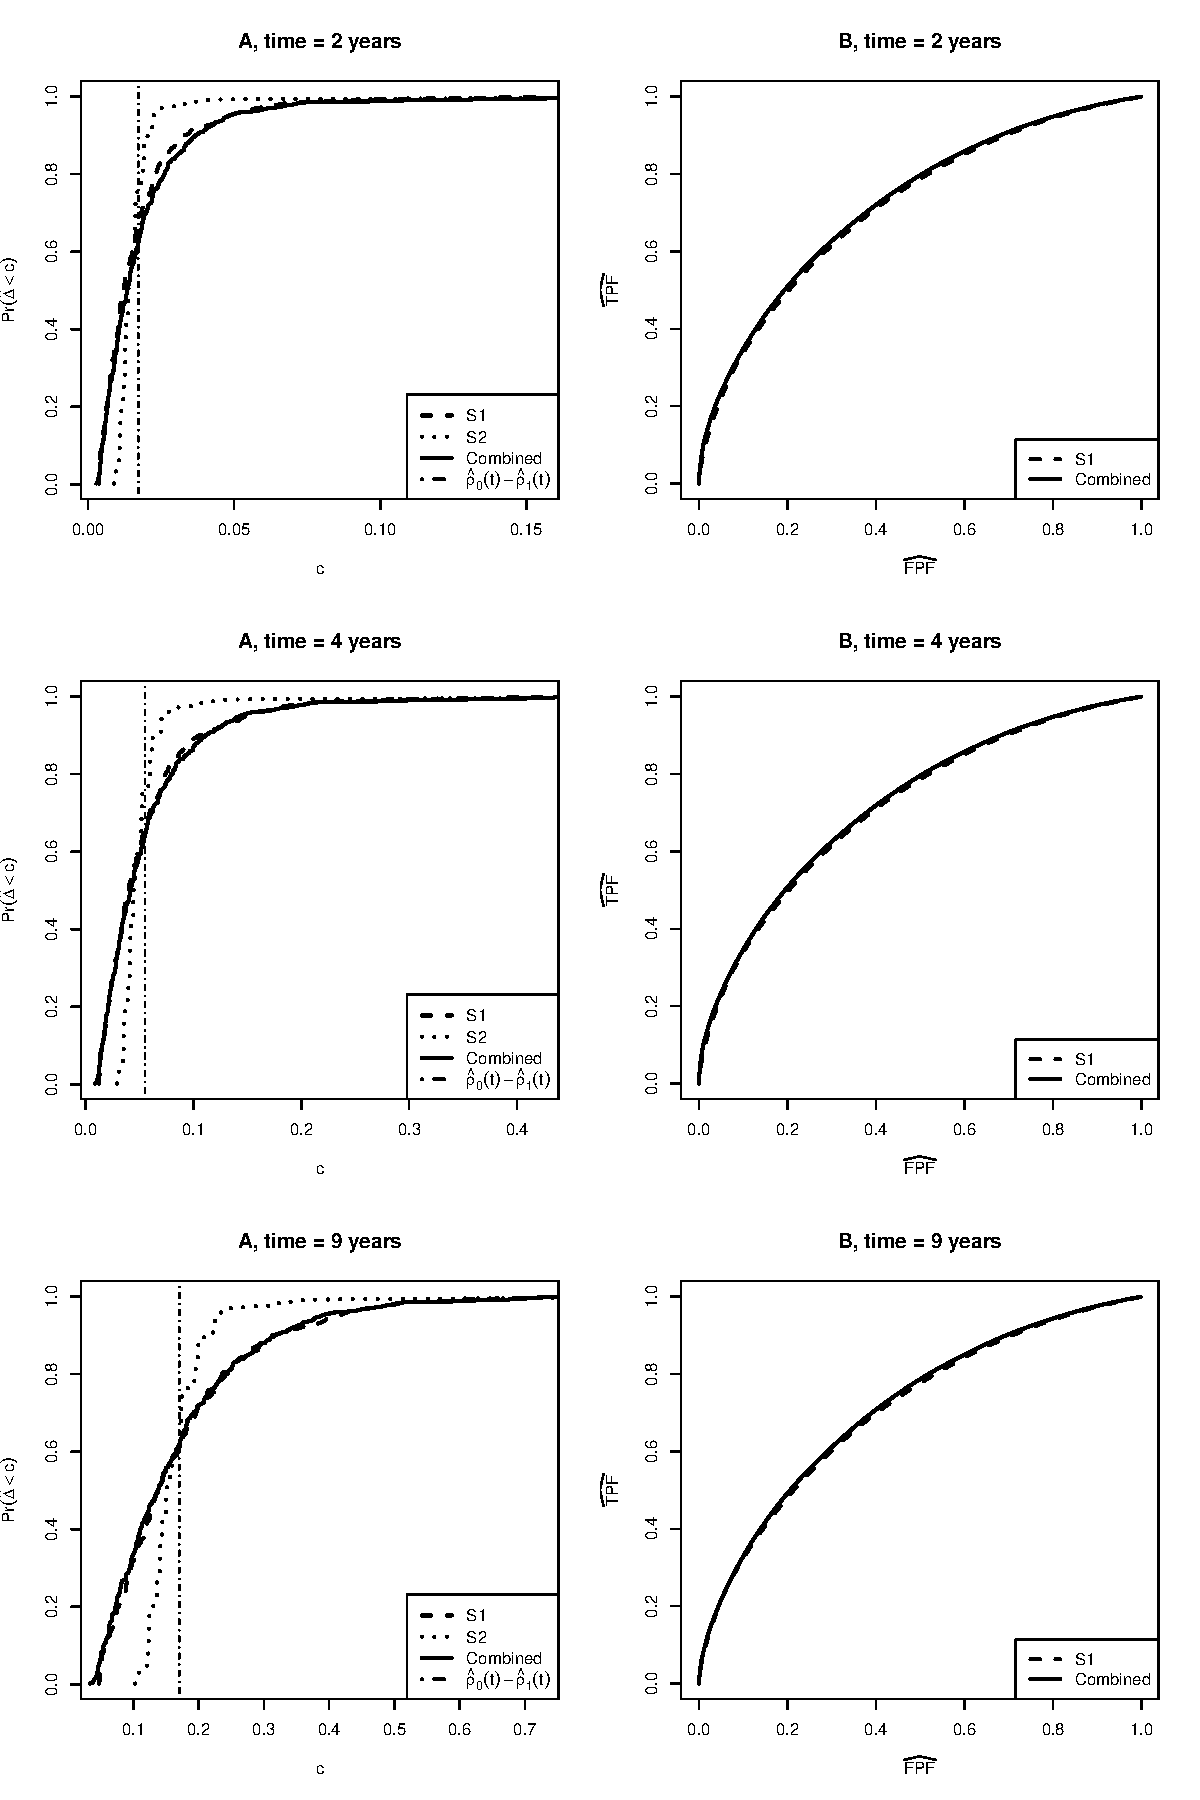
\includegraphics[scale=0.65]{dcct-figure-supplement-new-11-18-2013.pdf}
\end{center}
\caption{The A panels depict the estimated $CDF^{6.5}(c)$ versus $c$ for the truncated univariate candidate principal surrogates HBA1C and EGFR as well as for the combination candidate PS for given time points. The B panels depict the estimated $ROC^{6.5}(q)$ versus $q$ for HBA1C and the combination of HBA1C and EGFR at given time points. \label{exp}}
\end{figure}






\bibliographystyle{plainnat}
\bibliography{bib_dissertation}






\end{document}
